


\tikzset{every picture/.style={line width=0.75pt}} %set default line width to 0.75pt        

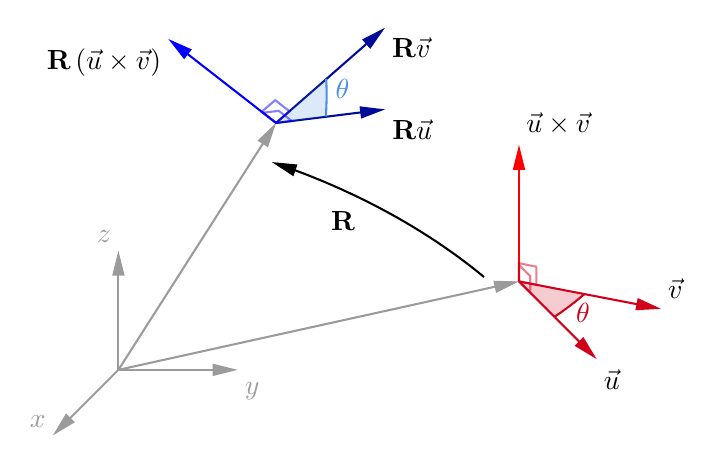
\begin{tikzpicture}[x=0.75pt,y=0.75pt,yscale=-1,xscale=1]
%uncomment if require: \path (0,268); %set diagram left start at 0, and has height of 268

%Straight Lines [id:da7480929076055294] 
\draw [color={rgb, 255:red, 155; green, 155; blue, 155 }  ,draw opacity=1 ]   (82,226) -- (137.4,226) ;
\draw [shift={(139.4,226)}, rotate = 180] [fill={rgb, 255:red, 155; green, 155; blue, 155 }  ,fill opacity=1 ][line width=0.08]  [draw opacity=0] (12,-3) -- (0,0) -- (12,3) -- cycle    ;
%Straight Lines [id:da13565413973667217] 
\draw [color={rgb, 255:red, 155; green, 155; blue, 155 }  ,draw opacity=1 ]   (82,226) -- (82,170.6) ;
\draw [shift={(82,168.6)}, rotate = 90] [fill={rgb, 255:red, 155; green, 155; blue, 155 }  ,fill opacity=1 ][line width=0.08]  [draw opacity=0] (12,-3) -- (0,0) -- (12,3) -- cycle    ;
%Straight Lines [id:da18952961905679389] 
\draw [color={rgb, 255:red, 155; green, 155; blue, 155 }  ,draw opacity=1 ]   (82,226) -- (51.81,256.19) ;
\draw [shift={(50.4,257.6)}, rotate = 315] [fill={rgb, 255:red, 155; green, 155; blue, 155 }  ,fill opacity=1 ][line width=0.08]  [draw opacity=0] (12,-3) -- (0,0) -- (12,3) -- cycle    ;
%Straight Lines [id:da8805177002425553] 
\draw [color={rgb, 255:red, 208; green, 2; blue, 27 }  ,draw opacity=1 ]   (275,183.4) -- (341.44,196.22) ;
\draw [shift={(343.4,196.6)}, rotate = 190.92] [fill={rgb, 255:red, 208; green, 2; blue, 27 }  ,fill opacity=1 ][line width=0.08]  [draw opacity=0] (12,-3) -- (0,0) -- (12,3) -- cycle    ;
%Straight Lines [id:da9953207458084412] 
\draw [color={rgb, 255:red, 255; green, 0; blue, 0 }  ,draw opacity=1 ]   (275,183.4) -- (275,119.6) ;
\draw [shift={(275,117.6)}, rotate = 90] [fill={rgb, 255:red, 255; green, 0; blue, 0 }  ,fill opacity=1 ][line width=0.08]  [draw opacity=0] (12,-3) -- (0,0) -- (12,3) -- cycle    ;
%Straight Lines [id:da697419604837394] 
\draw [color={rgb, 255:red, 208; green, 2; blue, 27 }  ,draw opacity=1 ]   (275,183.4) -- (310.99,219.39) ;
\draw [shift={(312.4,220.8)}, rotate = 225] [fill={rgb, 255:red, 208; green, 2; blue, 27 }  ,fill opacity=1 ][line width=0.08]  [draw opacity=0] (12,-3) -- (0,0) -- (12,3) -- cycle    ;
%Shape: Arc [id:dp795997683183645] 
\draw  [draw opacity=0][fill={rgb, 255:red, 208; green, 2; blue, 27 }  ,fill opacity=0.2 ] (306.55,189.44) .. controls (302.09,193.31) and (297.24,197) .. (292.19,200.39) -- (275,183.4) -- cycle ; \draw  [color={rgb, 255:red, 208; green, 2; blue, 27 }  ,draw opacity=1 ] (306.55,189.44) .. controls (302.09,193.31) and (297.24,197) .. (292.19,200.39) ;  
%Straight Lines [id:da7984648507315177] 
\draw [color={rgb, 255:red, 155; green, 155; blue, 155 }  ,draw opacity=1 ]   (82,226) -- (273.05,183.83) ;
\draw [shift={(275,183.4)}, rotate = 167.55] [fill={rgb, 255:red, 155; green, 155; blue, 155 }  ,fill opacity=1 ][line width=0.08]  [draw opacity=0] (12,-3) -- (0,0) -- (12,3) -- cycle    ;
%Straight Lines [id:da7735329414277254] 
\draw [color={rgb, 255:red, 155; green, 155; blue, 155 }  ,draw opacity=1 ]   (82,226) -- (156.89,108.73) ;
\draw [shift={(157.97,107.04)}, rotate = 122.56] [fill={rgb, 255:red, 155; green, 155; blue, 155 }  ,fill opacity=1 ][line width=0.08]  [draw opacity=0] (12,-3) -- (0,0) -- (12,3) -- cycle    ;
%Shape: Arc [id:dp9732073903623295] 
\draw  [draw opacity=0] (155.96,125.9) .. controls (194.23,138.66) and (230.23,158.07) .. (258.13,181.27) -- (131.79,226) -- cycle ; \draw    (158.25,126.68) .. controls (195.67,139.44) and (230.78,158.53) .. (258.13,181.27) ;  \draw [shift={(155.96,125.9)}, rotate = 19.43] [fill={rgb, 255:red, 0; green, 0; blue, 0 }  ][line width=0.08]  [draw opacity=0] (12,-3) -- (0,0) -- (12,3) -- cycle    ;
%Shape: Parallelogram [id:dp9828081717947923] 
\draw  [color={rgb, 255:red, 208; green, 2; blue, 27 }  ,draw opacity=0.5 ] (275,183.4) -- (275,175.4) -- (280.4,180.81) -- (280.4,188.81) -- cycle ;
%Shape: Parallelogram [id:dp8799263166271469] 
\draw  [color={rgb, 255:red, 208; green, 2; blue, 27 }  ,draw opacity=0.5 ] (275,183.33) -- (275,174.6) -- (283.4,176.32) -- (283.4,185.05) -- cycle ;
%Straight Lines [id:da8952339044508235] 
\draw [color={rgb, 255:red, 0; green, 12; blue, 153 }  ,draw opacity=1 ]   (157.97,107.04) -- (208.9,62.5) ;
\draw [shift={(210.41,61.19)}, rotate = 138.83] [fill={rgb, 255:red, 0; green, 12; blue, 153 }  ,fill opacity=1 ][line width=0.08]  [draw opacity=0] (12,-3) -- (0,0) -- (12,3) -- cycle    ;
%Straight Lines [id:da8008440479094254] 
\draw [color={rgb, 255:red, 0; green, 0; blue, 255 }  ,draw opacity=1 ]   (157.97,107.04) -- (107.63,67.84) ;
\draw [shift={(106.05,66.61)}, rotate = 37.91] [fill={rgb, 255:red, 0; green, 0; blue, 255 }  ,fill opacity=1 ][line width=0.08]  [draw opacity=0] (12,-3) -- (0,0) -- (12,3) -- cycle    ;
%Straight Lines [id:da2802924438933301] 
\draw [color={rgb, 255:red, 0; green, 12; blue, 153 }  ,draw opacity=1 ]   (157.97,107.04) -- (208.47,100.76) ;
\draw [shift={(210.45,100.51)}, rotate = 172.91] [fill={rgb, 255:red, 0; green, 12; blue, 153 }  ,fill opacity=1 ][line width=0.08]  [draw opacity=0] (12,-3) -- (0,0) -- (12,3) -- cycle    ;
%Shape: Arc [id:dp034042061516837085] 
\draw  [draw opacity=0][fill={rgb, 255:red, 74; green, 144; blue, 226 }  ,fill opacity=0.2 ] (182.11,85.86) .. controls (182.43,91.76) and (182.36,97.85) .. (181.93,103.92) -- (157.97,107.04) -- cycle ; \draw  [color={rgb, 255:red, 74; green, 144; blue, 226 }  ,draw opacity=1 ] (182.11,85.86) .. controls (182.43,91.76) and (182.36,97.85) .. (181.93,103.92) ;  
%Shape: Parallelogram [id:dp9451524906369364] 
\draw  [color={rgb, 255:red, 10; green, 0; blue, 255 }  ,draw opacity=0.5 ] (157.97,107.04) -- (151.65,102.13) -- (159.24,101.19) -- (165.55,106.1) -- cycle ;
%Shape: Parallelogram [id:dp17856130979854812] 
\draw  [color={rgb, 255:red, 10; green, 0; blue, 255 }  ,draw opacity=0.5 ] (157.91,107) -- (151.02,101.63) -- (157.54,96.06) -- (164.43,101.43) -- cycle ;

% Text Node
\draw (183,148.4) node [anchor=north west][inner sep=0.75pt]    {$\mathbf{R}$};
% Text Node
\draw (314.4,224.2) node [anchor=north west][inner sep=0.75pt]    {$\vec{u}$};
% Text Node
\draw (345.4,193.2) node [anchor=south west] [inner sep=0.75pt]    {$\vec{v}$};
% Text Node
\draw (277,114.2) node [anchor=south west] [inner sep=0.75pt]    {$\vec{u} \times \vec{v}$};
% Text Node
\draw (212.45,103.91) node [anchor=north west][inner sep=0.75pt]    {$\mathbf{R}\vec{u}$};
% Text Node
\draw (212.41,64.59) node [anchor=north west][inner sep=0.75pt]    {$\mathbf{R}\vec{v}$};
% Text Node
\draw (104.05,70.01) node [anchor=north east] [inner sep=0.75pt]    {$\mathbf{R}\left(\vec{u} \times \vec{v}\right)$};
% Text Node
\draw (301,192.4) node [anchor=north west][inner sep=0.75pt]  [color={rgb, 255:red, 208; green, 2; blue, 27 }  ,opacity=1 ]  {$\theta $};
% Text Node
\draw (185.19,84.51) node [anchor=north west][inner sep=0.75pt]  [color={rgb, 255:red, 74; green, 144; blue, 226 }  ,opacity=1 ]  {$\theta $};
% Text Node
\draw (48.4,255.2) node [anchor=south east] [inner sep=0.75pt]  [color={rgb, 255:red, 155; green, 155; blue, 155 }  ,opacity=1 ]  {$x$};
% Text Node
\draw (141.4,230.4) node [anchor=north west][inner sep=0.75pt]  [color={rgb, 255:red, 155; green, 155; blue, 155 }  ,opacity=1 ]  {$y$};
% Text Node
\draw (80,166.2) node [anchor=south east] [inner sep=0.75pt]  [color={rgb, 255:red, 155; green, 155; blue, 155 }  ,opacity=1 ]  {$z$};


\end{tikzpicture}
